\documentclass[10pt,twocolumn,letterpaper]{article}

\usepackage{cvpr}
\usepackage{times}
\usepackage{epsfig}
\usepackage{graphicx}
\usepackage{booktabs}
\usepackage{amsmath}
\usepackage{amssymb}
\usepackage[pagebackref,breaklinks,colorlinks,allcolors=blue]{hyperref}
\usepackage{tikz}
\usetikzlibrary{arrows.meta,positioning,calc}
\usepackage{enumitem}
\usepackage{xspace}
\usepackage{float}

\cvprfinalcopy

\def\cvprPaperID{****}
\def\confName{CSE 252D}
\def\confYear{Spring 2026}

\begin{document}

\title{AutoPass-Gen: Scenario Generation for Evaluating Urgency-Aware Passing Decisions in CARLA}

\author{
Rohan Sachdeva \quad Xinwei Mai \quad Pranav Prabu \quad Rathang Pandit \\
University of California, San Diego \\
{\tt\small \{rosachdeva, xmai, pprabu, rpandit\}@ucsd.edu}
}

\maketitle

\section{Problem}
Autonomous driving systems are often evaluated on fixed routes, random traffic, or a small set of hand-designed scenarios. These evaluations can miss rare failures because the simulator is not actively searching for situations where a driving policy makes the wrong decision. We focus on one concrete and safety-critical maneuver: \textbf{passing a slow lead vehicle}. The ego vehicle must decide whether to wait, pass, or replan while reasoning about front distance, rear traffic, oncoming gaps, visibility, road geometry, sensor reliability, and user urgency.

We study \textbf{scenario generation for urgency-aware passing}. Each generated case contains both CARLA world facts, such as route, traffic, occlusion, and weather, and a synthetic travel request, such as ``I need to arrive in 10 minutes,'' The request is not meant to require a full chatbot; instead it gives the agent a structured context from which to infer start, goal, deadline, urgency level, and delay cost. Our goal is to generate CARLA scenarios that stress-test whether a driving system can safely trade off progress and risk. The core research question is: \emph{under what generated conditions does urgency cause a passing policy to become unsafe, over-conservative, or inconsistent?}

\section{Motivation}
Several autonomous driving projects focus on perception, navigation, or low-level control. Our project is different: we focus on \textbf{generation-driven evaluation}. Passing is narrow enough to implement in CARLA but rich enough to expose meaningful failures. A fully conservative agent may never pass and therefore fail time-sensitive tasks; an urgency-driven agent may pass in unsafe gaps. The interesting behavior lies at the boundary.

Xinwei's decision diagram~\ref{fig:PDD} motivates our policy loop. To avoid requiring a real-time chatbot, the Scenario Generator produces a synthetic travel request together with the CARLA scene. A Request/Urgency Interpreter then extracts the start, goal, deadline, urgency level, and delay cost from this request. The ego vehicle follows a normal route and enters the passing loop only when a slow front vehicle blocks progress. The loop repeatedly evaluates the current state, uses tools such as RGB/depth perception, SLAM/map state, segmentation, and safety checking, and then chooses \texttt{pass}, \texttt{wait}, or \texttt{replan}. This gives us a concrete agentic system with tool use, self-correction, and measurable outcomes.

\begin{figure}
    \centering
    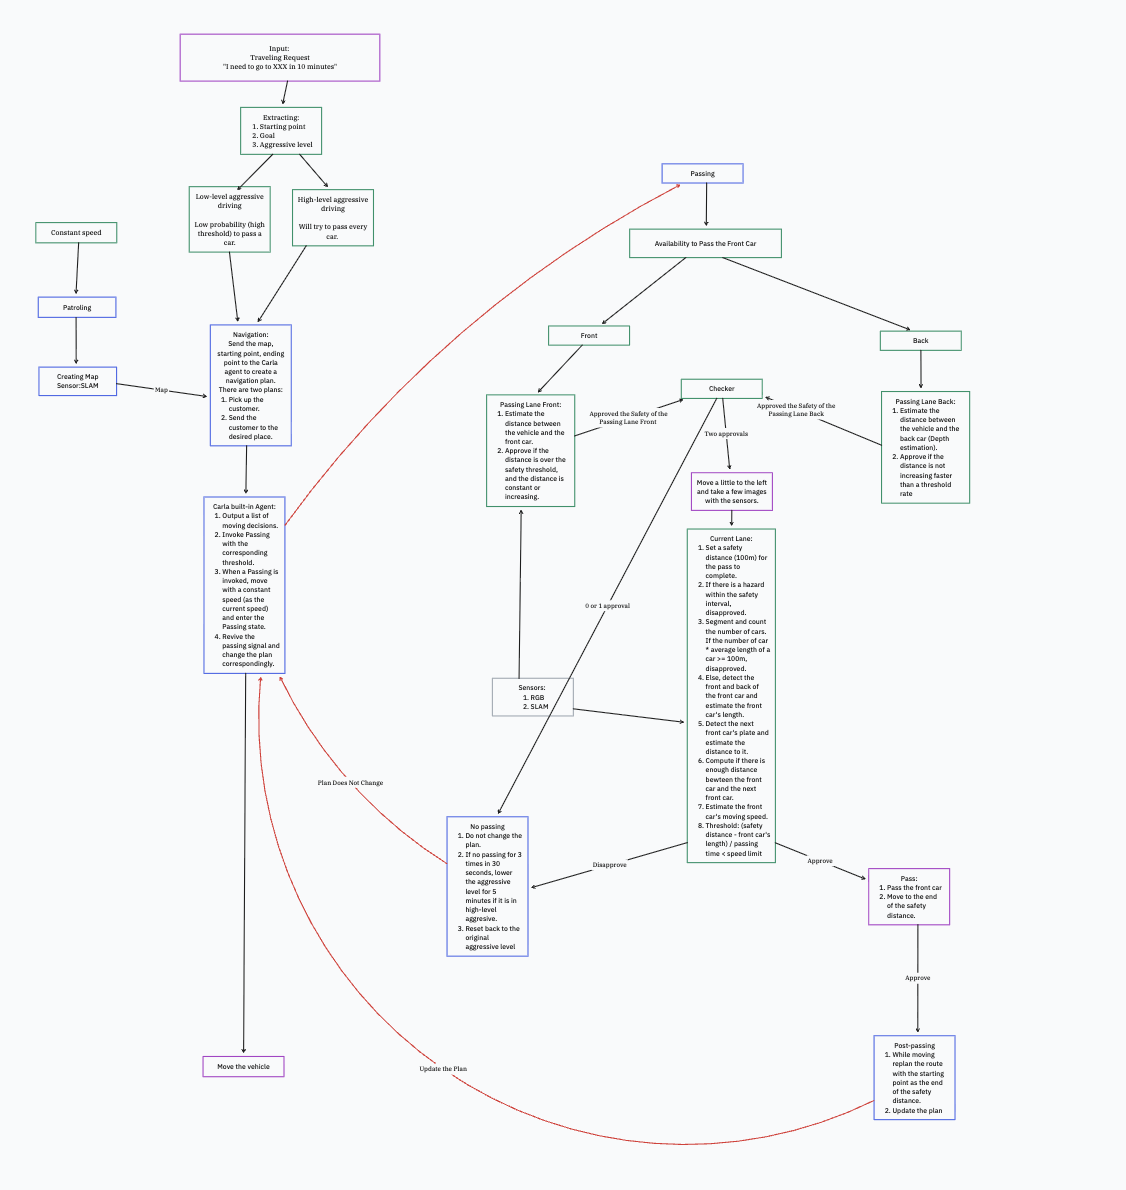
\includegraphics[width=0.5\linewidth]{passing-diagram.png}
    \caption{Urgency-Aware Passing Decision Diagram. The diagram shows how a generated travel request and CARLA scene are converted into an urgency-aware passing loop. Blue boxes indicate major stages, green boxes indicate agent reasoning or checking steps, and purple boxes indicate inputs, outputs, or actions.}
    \label{fig:PDD}
\end{figure}


\section{Key Background Literature}
We use CARLA~\cite{dosovitskiy2017carla} because it provides repeatable urban environments, configurable weather, dynamic actors, and access to RGB/depth sensors and simulator state. Prior work on conditional imitation learning~\cite{codevilla2018conditional} and privileged training~\cite{chen2019learning} studies how policies can learn to drive from data or privileged information. However, these works do not directly answer which safety-critical scenarios should be generated to expose policy weaknesses.

Our work is closer to adversarial testing and falsification: rather than only training a policy, we generate situations that reveal failures. The contribution is a compact passing scenario representation, a closed-loop scenario generator, and an interpretable urgency-aware passing policy whose decisions can be audited through distances, gaps, urgency, visibility, and critic approvals.

\section{Method Overview}
AutoPass-Gen evaluates urgency-aware passing as a closed-loop generation and testing problem. Each trial begins with a structured \texttt{ScenarioSpec} containing route information, a synthetic travel request, ego/lead/rear/oncoming traffic, occlusion, weather, and sensor settings. The request is interpreted into a deadline, urgency level, and delay cost. The ego vehicle then follows a route until it encounters a slow lead vehicle, at which point the passing loop begins.

At each timestep, the Perception/Map module estimates the current \texttt{PassState}, including front distance, rear distance, oncoming distance, relative speeds, visibility, deadline pressure, and urgency. The Passing Agent proposes one of three actions: \texttt{pass}, \texttt{wait}, or \texttt{replan}. The Safety Checker accepts or rejects passing proposals using time-to-collision, rear-gap, oncoming-gap, front-gap, and visibility constraints. Approved decisions are sent to the Execution module, while rejected decisions are converted into safer wait or replan behavior. The Evaluator records collisions, route completion, time-to-goal, pass attempts, unsafe passes, minimum TTC, and the final failure category.

AutoPass-Gen has three coupled components: a \textbf{scenario generator}, a \textbf{request/urgency interpreter}, and an \textbf{urgency-aware passing policy}. The generator creates difficult passing cases and synthetic travel requests; the interpreter converts those requests into route and urgency variables; and the policy is the system being evaluated during closed-loop driving. The key research idea is that the Scenario Generator is not passive: rollout failures can be used to mutate future scenarios toward narrower gaps, stronger occlusions, tighter deadlines, and more difficult traffic configurations.

\subsection{Scenario Representation}
We represent each case as a structured specification:
\begin{align*}
\texttt{ScenarioSpec} = \{&\texttt{map}, \texttt{route}, \texttt{request}, \texttt{ego}, \\
&\texttt{lead}, \texttt{rear}, \texttt{oncoming}, \\
&\texttt{occlusion}, \texttt{weather}, \texttt{sensor} \}.
\end{align*}
Here, \texttt{request} contains a synthetic travel instruction with a start, goal, deadline, and optional natural-language reason for urgency. The generator creates this request but does not directly decide the policy's risk tolerance. Instead, the Request/Urgency Interpreter maps the request to an urgency level and delay cost. The remaining fields define the physical scene: \texttt{lead} controls the front vehicle distance, speed, and acceleration; \texttt{rear} controls whether lane change is safe from behind; \texttt{oncoming} controls the available passing gap; \texttt{occlusion} models parked cars, curves, junctions, or limited sight distance; and \texttt{weather} changes RGB reliability. This is higher-level than raw CARLA scripts but lower-level than unrestricted natural language, making scenarios easy to instantiate, perturb, log, and compare.
% ; and \texttt{urgency} changes the delay penalty without removing hard safety constraints. 


\subsection{Request and Urgency Interpretation}
A key design choice is that the generator creates the initial facts, while the agentic system performs the interpretation. For example, the generator may create a request such as ``drive from A to B and arrive within 10 minutes'' together with a CARLA scene containing a slow lead vehicle, rear traffic, and an oncoming gap. The Request/Urgency Interpreter then computes structured variables such as
\begin{align*}
\texttt{start},\quad \texttt{goal},\quad \texttt{deadline},\quad \\
\texttt{urgency\_level},\quad \texttt{delay\_cost}.
\end{align*}
This avoids requiring a real user-facing chatbot while preserving the agentic reasoning step: urgency is inferred from the generated request rather than directly hard-coded as the final policy decision. During rollout, the agent repeatedly evaluates the current state, proposes \texttt{pass}, \texttt{wait}, or \texttt{replan}, executes the approved action, and then reevaluates the updated state.

\subsection{Scenario Generation Loop}
The generator samples or mutates \texttt{ScenarioSpec} values to create increasingly difficult cases: slow lead vehicles, deceptive oncoming gaps, unsafe rear vehicles, occlusions, weather changes that require sensor-mode adaptation, and deadlines that induce different levels of urgency. After each rollout, the evaluator returns safety and efficiency metrics. Failure cases are fed back into the generator, which increases difficulty by narrowing gaps, increasing occlusion, changing traffic timing, tightening deadlines, or changing the route context. The generator therefore controls the experimental distribution, while the agent still performs the interpretation and decision-making during rollout.

\subsection{Urgency-Aware Passing Policy}
The ego vehicle follows a CARLA baseline agent until it detects a slow lead vehicle. The passing loop then estimates front distance, rear distance, relative velocity, visibility, and oncoming traffic. It approves a pass only when two conditions hold: (i) the maneuver improves progress under the current urgency, and (ii) geometric and temporal safety margins remain valid. A simplified safety check is
\[
d_{\mathrm{gap}} >
v_{\mathrm{ego}}t_{\mathrm{pass}}
+\frac{1}{2}a_{\mathrm{ego}}t_{\mathrm{pass}}^2+\Delta,
\]
where \(d_{\mathrm{gap}}\) is available distance before conflict, \(t_{\mathrm{pass}}\) is estimated passing time, and \(\Delta\) is a safety buffer. Urgency may lower the threshold for considering a pass, but it cannot override collision risk, insufficient visibility, or unsafe rear traffic.

% \newpage

\section{System Architecture}
\begin{figure}[H]
\centering
\resizebox{\linewidth}{!}{
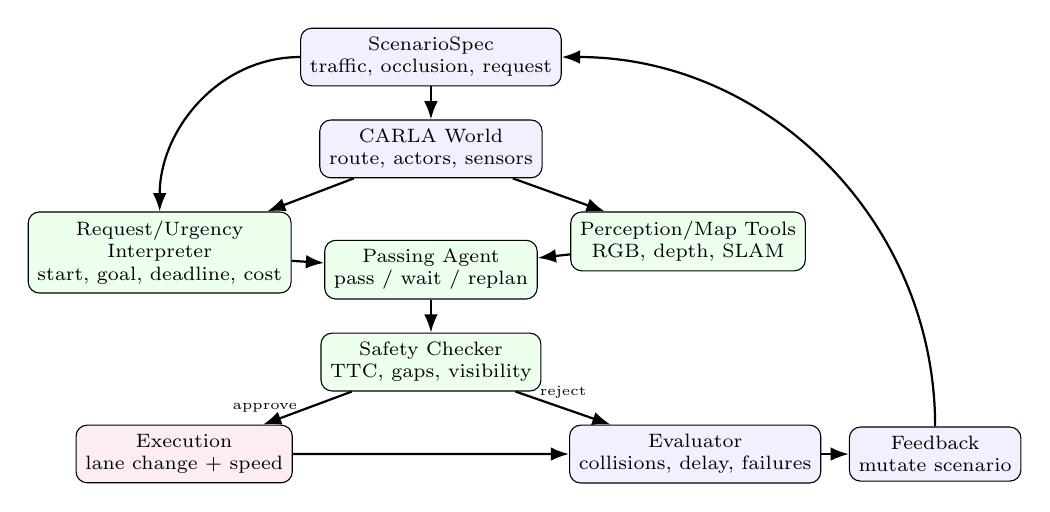
\begin{tikzpicture}[
node distance=0.42cm and 0.35cm,
box/.style={draw, rounded corners, align=center, minimum width=1.95cm, minimum height=0.52cm, font=\scriptsize},
data/.style={box, fill=blue!6},
agent/.style={box, fill=green!7},
act/.style={box, fill=purple!7},
arrow/.style={-Latex, thick}
]
\node[data] (spec) {ScenarioSpec\\traffic, occlusion, request};
\node[data, below=of spec] (carla) {CARLA World\\route, actors, sensors};
\node[agent, below left=of carla] (parse) {Request/Urgency\\Interpreter\\start, goal, deadline, cost};
\node[agent, below right=of carla] (sense) {Perception/Map Tools\\RGB, depth, SLAM};
\node[agent, below=0.78cm of carla] (pass) {Passing Agent\\pass / wait / replan};
\node[agent, below=of pass] (critic) {Safety Checker\\TTC, gaps, visibility};
\node[act, below left=of critic] (control) {Execution\\lane change + speed};
\node[data, below right=of critic] (metrics) {Evaluator\\collisions, delay, failures};
\node[data, right=of metrics] (feedback) {Feedback\\mutate scenario};

\draw[arrow] (spec) -- (carla);
\draw[arrow] (spec.west) to[out=180,in=90] (parse.north);
\draw[arrow] (carla) -- (parse);
\draw[arrow] (carla) -- (sense);
\draw[arrow] (parse) -- (pass);
\draw[arrow] (sense) -- (pass);
\draw[arrow] (pass) -- (critic);
\draw[arrow] (critic) -- node[left,font=\tiny]{approve} (control);
\draw[arrow] (control) -- (metrics);
\draw[arrow] (critic) -- node[above,font=\tiny]{reject} (metrics);
\draw[arrow] (metrics) -- (feedback);
\draw[arrow] (feedback.north) to[out=90,in=0] (spec.east);
\end{tikzpicture}
}
\vspace{-6pt}
\caption{AutoPass-Gen architecture. The main research object is the closed-loop generation and evaluation of passing scenarios; the passing agent provides an interpretable policy to test.}
\vspace{-10pt}
\label{AutoPassArch}
\end{figure}

\section{Working Prototype Details}
We implemented an initial Python prototype of the full AutoPass-Gen architecture. The current prototype is \textbf{simulator-independent}: it uses a lightweight kinematic rollout backend rather than CARLA so that we can validate the scenario generation, urgency interpretation, passing policy, safety checking, logging, and evaluation loop before all team members need to run CARLA. This is not intended to replace CARLA; rather, it gives us a stable integration target whose world-state and execution interfaces can be swapped for CARLA actor spawning, sensors, and controls.

The prototype implements the major components in Figure~\ref{AutoPassArch}. The \textbf{Scenario DSL} stores each generated case as a typed \texttt{ScenarioSpec}. The \textbf{Scenario Generator} samples deadlines, lead vehicle speeds, rear traffic, oncoming gaps, occlusion levels, weather, and sensor modes. The \textbf{Request/Urgency Interpreter} converts synthetic travel requests into structured urgency variables. The \textbf{Perception/Map Tools} estimate front distance, rear distance, oncoming distance, visibility, and relative speeds using privileged or noisy sensor-like state. The \textbf{Passing Agent} proposes \texttt{plan}, \texttt{wait}, or \texttt{replan}. The \textbf{Safety Checker} rejects unsafe passes using TTC, rear-gap, oncoming-gap, front-gap, and visibility constraints. The \textbf{Execution Agent} updates the ego state with a simple kinematic modl, and the \textbf{Evaluator} writes per-timestep traces and aggregate metrics.

The prototype also includes three policy variants: \textbf{AutoPass}, our urgency-aware passing policy; \textbf{no-pass}, a conservative baseline that never attempts passing; and \textbf{aggressive}, a progress-seeking baseline that attempts risky passes. Each rollout produces a JSON trace containing distances, visibility, urgency, decision, risk score, critic approval, and reason strings, as well as a CSV row containing collision status, route completion, time-to-goal, pass attempts, unsafe passes, minimum TTC, and failure type. The failure taxonomy currently includes \texttt{unsafe\_pass}, \texttt{missed\_safe\_pass}, \texttt{over\_conservative\_delay}, \texttt{sensor\_mode\_failure}, and \texttt{collision}.

\section{Initial Results and Observations}
We evaluated the local prototype on 50 generated passing scenarios using the three policies described above. These results should be interpreted as an integration and debugging checkpoint rather than a final CARLA evaluation. The purpose is to test whether the full AutoPass-Gen loop produces meaningful safety-efficiency tradeoffs before replacing the lightweight backend with CARLA.

\begin{table}[t]
    \centering
    \small
    \begin{tabular}{lrrrr}
         \toprule
         Policy & Failures & Avg. time (s) & Pass attempts & Unsafe passes \\
         \midrule
         No-pass & 16/50 & 96.58 & 0 & 0 \\
         AutoPass & 13/50 & 90.16 & 19 & 0 \\
         Aggressive & 41/50 & 60.08 & 154 & 134 \\
         \bottomrule
    \end{tabular}
    \vspace{-4pt}
    \caption{Initial local evaluation over 50 generated scenarios. AutoPass attempts selected passes and reduces delay relative to non-pass while avoiding unsafe passes. The aggressive baseline is faster but produces many unsafe passes.}
    \label{tab:initial-results}
    \vspace{-8pt}
\end{table}

Table~\ref{tab:initial-results} shows the intended qualitative behavior. The no-pass baseline never attempts a pass and produces no unsafe-pass failures, but it has the highest average time-to-goal and produces 16 over-conservative delay failures. The aggressive baseline achieves the lowest average time-to-goal, but fails in 41 out of 50 scenarios, mostly through unsafe passes. AutoPass produces an intermediate behavior: it attempts passes selectively, has zero unsafe-pass failures, reduces over-conservative delay failures from 16 to 11 relative to no-pass, and reduces average time-to-goal from 96.58s to 90.16s.

\begin{table}[t]
    \centering
    \small
    \begin{tabular}{lrrrr}
         \toprule
         Policy & None & Delay & Missed safe pass & Unsafe pass \\
         \midrule
         No-pass & 34 & 16 & 0 & 0 \\
         AutoPass & 37 & 11 & 2 & 0 \\
         Aggressive & 9 & 2 & 0 & 39 \\
         \bottomrule
    \end{tabular}
    \vspace{-4pt}
    \caption{Failure type distribution for the 50-scenario local evaluation. AutoPass avoids unsafe passes while reducing conservative-delay failures relative to no-pass.}
    \label{tab:failure-types}
    \vspace{-8pt}
\end{table}

The failure breakdown in Table~\ref{tab:failure-types} supports the main project hypothesis. Generated urgent passing scenarios expose the tradeoff between progress and safety: a policy that never passes avoids unsafe behavior but can miss deadlines, while a policy that aggressively pursues progress frequently chooses unsafe gaps. AutoPass lies between these extremes by using urgency to consider passing, while still allowing the Safety Checker to reject proposals with insufficient TTC, poor visibility, unsafe rear traffic, or inadequate oncoming gap.

The trace format was also useful for debugging the prototype. Early local runs revealed two backed issues: oncoming vehicles were initially counted as collisions even when the ego vehicle was not in the passing lane, and waiting behind a lead vehicle initially lacked safe car-following behavior. We fixed these by making collision checks lane-aware, computing distances from explicit actor positions, and adding adaptive cruise-control-like following behavior for wait and replan actions. These fixes make the local prototype suitable for generating initial metrics and interpretable traces while the next phase connects the same interfaces to CARLA.

\section{Representations and Proposed DSL}
Generated scenarios will be implemented as compact JSON-like objects:
\[
\begin{small}
\begin{array}{l}
\texttt{\{}\\
\quad \texttt{request: \{text, start, goal, deadline\},}\\
\quad \texttt{route: \{town, start, goal, lane\_type\},}\\
\quad \texttt{lead: \{distance, speed, accel\},}\\
\quad \texttt{rear: \{distance, speed\},}\\
\quad \texttt{oncoming: \{distance, speed, gap\_time\},}\\
\quad \texttt{occlusion: \{type, severity, sight\_distance\},}\\
\quad \texttt{weather: \{rain, fog, sun\_angle\},}\\
% \quad \texttt{urgency: \{level, deadline, delay\_cost\}}\\
\texttt{\}}
\end{array}
\end{small}
\]
The runtime state passed between agents is
\begin{align*}
\texttt{PassState} = \{&\texttt{ego}, \texttt{lead}, \texttt{rear}, \texttt{gap},\\
&\texttt{visibility}, \texttt{deadline},  \texttt{urgency}, \\
&\texttt{delay\_cost}, \texttt{decision}, \texttt{risk}\}
\end{align*}
Every rollout therefore produces not only a video and metric score, but also a trace explaining why the agent passed, waited, or replanned.

\section{Agent Roles}
Figure~\ref{AutoPassArch} shows the basic architecture for the experiment. The \textbf{Scenario Generator} proposes CARLA configurations and synthetic travel requests that stress passing. The \textbf{Request/Urgency Interpreter} extracts the route, deadline, urgency level, and delay cost from the generated request and world context. The \textbf{Perception/Map Tools} estimate distances, lane geometry, visibility, and traffic context from RGB, depth, SLAM, or simulator state. The \textbf{Passing Agent} proposes \texttt{pass}, \texttt{wait}, or \texttt{replan}. The \textbf{Safety Checker} rejects unsafe proposals using TTC, rear-gap, front-gap, and visibility constraints. The \textbf{Execution Agent} converts approved decisions into CARLA controls. The \textbf{Evaluator} logs metrics and sends failures back to the generator.

\section{Expected Outcomes}
The main expected outcome is a CARLA-backed version of the current AutoPass-Gen loop. The local prototype already implements the structured scenario representation, urgency interpretation, passing/no-passing policies, safety checking, trace logging, and metric evaluation. The remaining work is to replace the lightweight kinematic backend with CARLA actor spawning, map-based routes, sensors, and vehicle controls.

Our next milestone is a minimal CARLA scenario in which a \texttt{ScenarioSpec} spawns an ego vehicle, slow lead vehicle, rear vehicle, and oncoming vehicle on a two-lane route. We will first use simulator state for distances and traffic context, then add RGB/depth-based estimates for selected quantities if time permits. The final evaluation will compare AutoPass against the no-pass and aggressive baselines on a small suite of generated CARLA scenarios.

By the final report, we aim to deliver: (1) a structured scenario generator for controlled passing stress tests, (2) an urgency-aware passing baseline with interpretable traces, (3) quantitative comparison against conservative and aggressive baselines, (4) a failure taxonomy covering unsafe pass, missed safe pass, over-conservative delay, sensor-mode failure, and collision, and (5) at least a small number of CARLA-backed examples with screenshots or videos. 

% Metrics include collision rate, route completion, time-to-goal, pass-attempt rate, unsafe-pass rate, minimum TTC, and number of generated failures. The final result should show that generated passing scenarios reveal policy weaknesses more efficiently than random traffic alone.

\section{Scope and Feasibility}
The project is scoped around generation-driven evaluation rather than building a full autonomous driving stack from scratch. Our current prototype deliberately separates the scenario, policy, safety, execution, and evaluation interfaces from the simulator backend. This lets us test the full decision loop locally while keeping CARLA integration focused and feasible. 

For the next phase, we will use CARLA's built-in agents, traffic manager, and simulator state where needed. The minimum CARLA-backed system only needs to instantiate a small number of passing scenarios, run the pass/wait/replan loop, and log traces using the same \texttt{ScenarioSpec} and \texttt{PassState} interfaces. If time permits, we will replace privileged state estimates with RGB/depth-based perception for selected quantities such as front distance, visibility, or vehicle presence. This preserves the main research contribution: generated scenarios that expose when urgency-aware passing policies become unsafe, over-conservative, or inconsistent.

\section{Team Plan}

To complete the project in the remaining weeks, we divide the work by interface boundaries. Rohan will own integration, evaluation, plotting, and report writing, ensuring that each module plugs into the shared \texttt{ScenarioSpec} and \texttt{PassState} formats. Xinwei will own the passing logic and Safety Checker, aligning the implemented pass/wait/replan loop with the decision diagram and producing policy pseudocode for the report. Pranav will own CARLA scenario instantiation, including actor spawning, map and route setup, weather, sensors, and a small number of working CARLA examples. Rathang will own perception/map tools, baseline comparisons, metrics, and summary plots.

The immediate Week 7 target is a minimal CARLA-backed scenario with one ego vehicle, one slow lead vehicle, and one oncoming vehicle. Week 8 will focus on comparisons and failure cases across AutoPass, no-pass, and aggressive policies. Week 9 will focus on final figures, trace examples, screenshots or videos, and report polish.

{\small
\vspace{-4pt}
\bibliographystyle{ieeenat_fullname}
\bibliography{refs}
}

\end{document}